\subsection{Màn hình Menu của Client}
\subsubsection{Mô tả}
Dưới đây là nội dung hiển thị của màn hình Menu tương ứng với vai trò \textbf{Admin} (\textbf{Client}). Ở màn hình menu của Client, ứng dụng hỗ trợ 2 chức năng cơ bản: Thêm một người dùng mới vào danh sách kết nối (nút \textbf{Add new user}), kết nối trực tiếp đến một người dùng nào đó (\textbf{Connect to user}). (Hình \ref{fig:ClientMenuWindow})
\begin{figure}[H]
	\centering{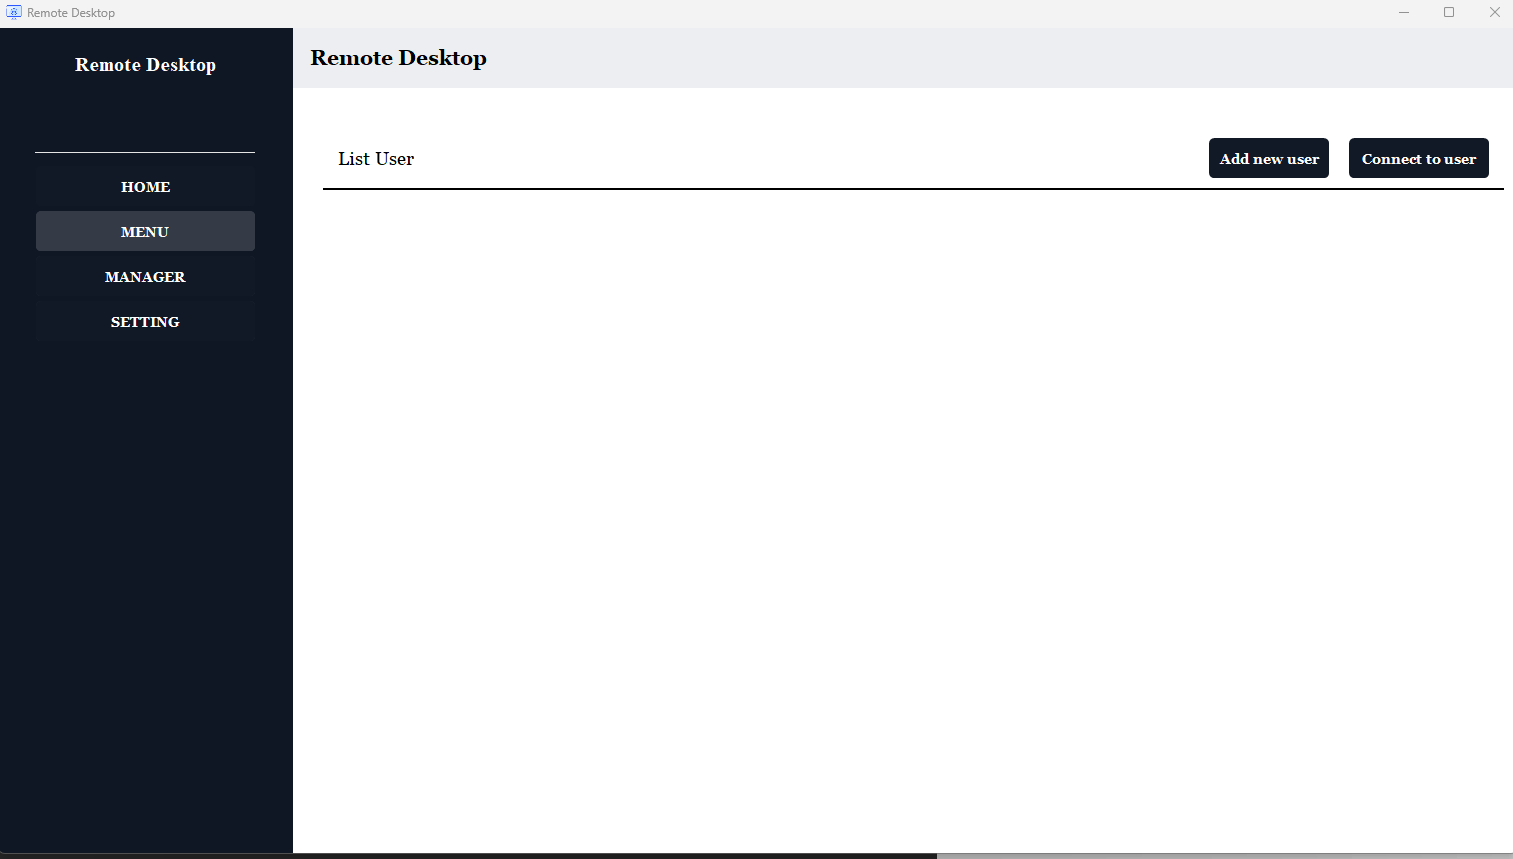
\includegraphics[scale=0.4]{ClientMenuWindow}}
	\caption{Màn hình chính của ứng dụng}
	\label{fig:ClientMenuWindow}
\end{figure}
\subsubsection{Thêm một người dùng mới vào danh sách các kết nối (nút Add new user)}
Khi ta sử dụng chức năng \textbf{Add new user}, hộp thoại \textbf{Add new user} xuất hiện với 2 trường thông tin cần nhập đó là ``User id'' và ``User IP Address''. Trường ``User id'' yêu cầu ta nhập tên nhận dạng, trường này có kiểu dữ liệu là \verb|std::string|, mục đích của việc điền thông tin này là để tạo lưu lại tên cụ thể trên danh sách các User nằm ở bên dưới để cho ta dễ nhận biết tên User ta muốn kết nối. Ở trường ``User IP Address'', ta nhập địa chỉ IP của máy cần được kết nối (Hình \ref{fig:AddNewUserBox}). 

\begin{figure}[H]
	\centering{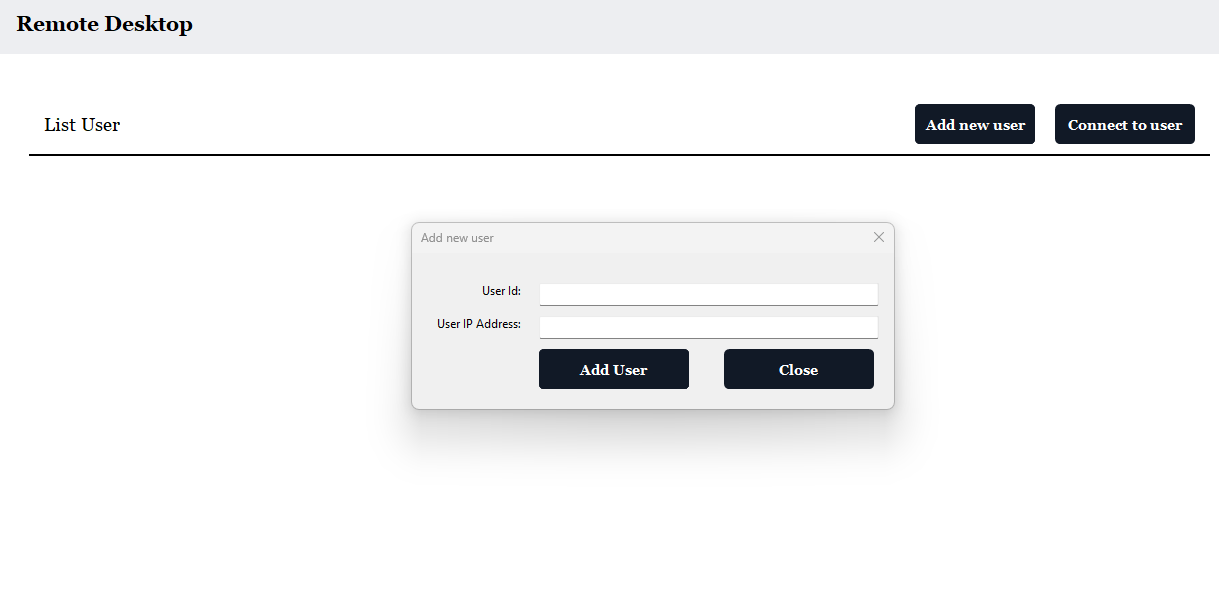
\includegraphics[scale=0.5]{AddNewUserBox}}
	\caption{Hộp thoại Add new user}
	\label{fig:AddNewUserBox}
\end{figure}

Sau khi nhập xong, ta ấn nút ``Add user'' ở góc trái để thêm một người dùng mới vào danh sách kết nối bên dưới. Sau khi thêm một vài người dùng vào danh sách kết nối thì màn hình Menu sẽ có hiển thị như sau. (Hình \ref{fig:UserList})

\begin{figure}[H]
	\centering{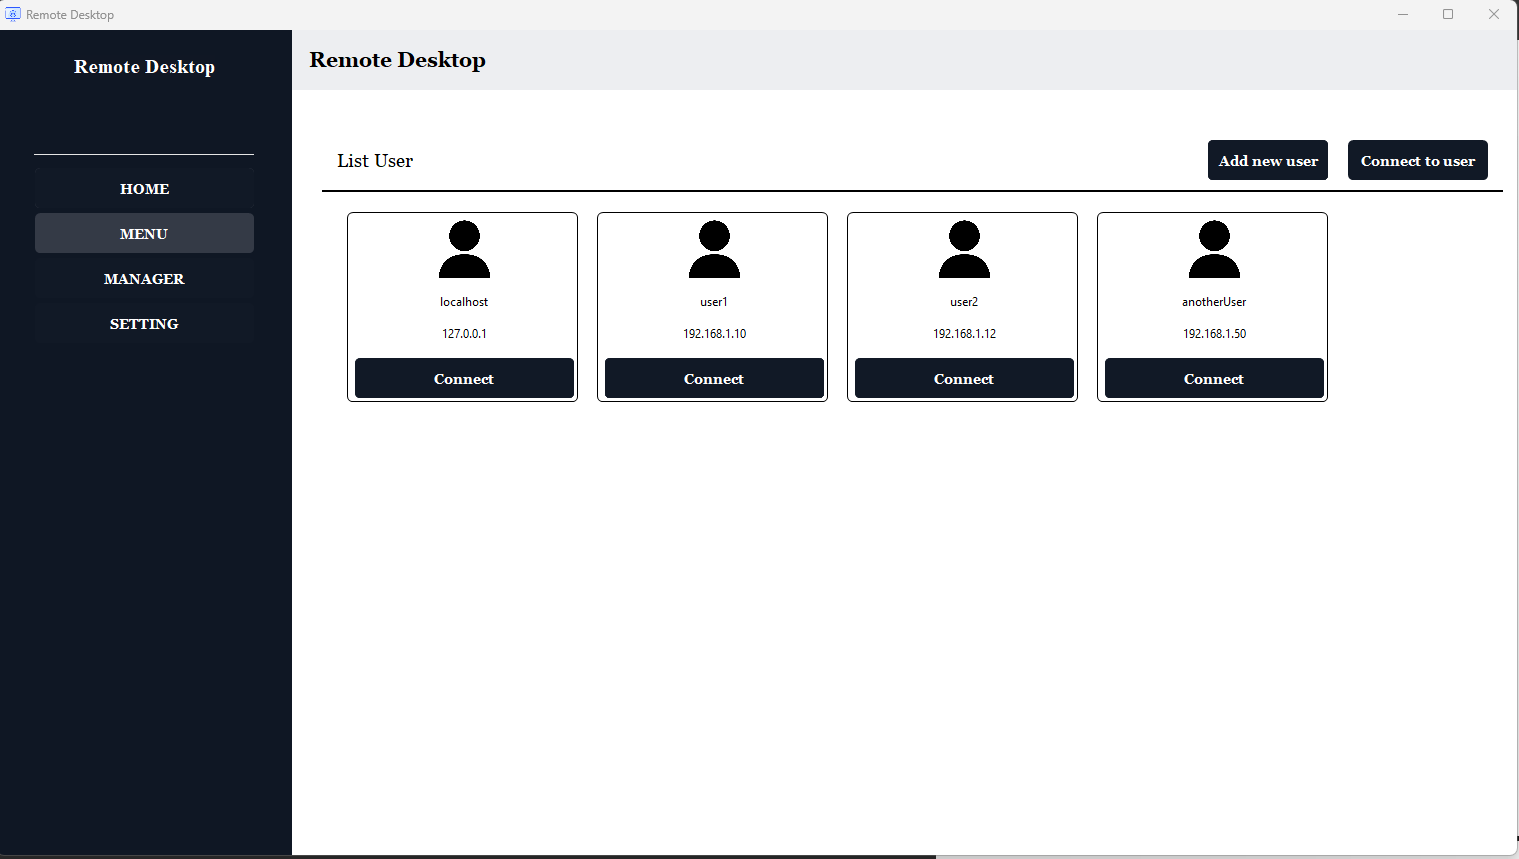
\includegraphics[scale=0.4]{UserList}}
	\caption{Danh sách các user sau khi nhập}
	\label{fig:UserList}
\end{figure}

\subsubsection{Kết nối đến Server (nút Connect/Connect to user)}
Để kết nối đến server, ta có 2 cách để thực hiện: Sử dụng nút ``Connect to user'' ngay bên cạnh ``Add new User'' hoặc nút ``Connect'' ngay bên dưới user tương ứng trong danh sách User trong hình \ref{fig:UserList}.

Nếu ta sử dụng lựa chọn ``Connect to user'', hộp thoại hiện lên với cấu trúc tương tự hộp thoại ``Add new user'', chỉ khác là ở góc trái hiển thị lựa chọn ``Connect to user''. (Hình \ref{fig:ConnectToUserBox})

\begin{figure}[H]
	\centering{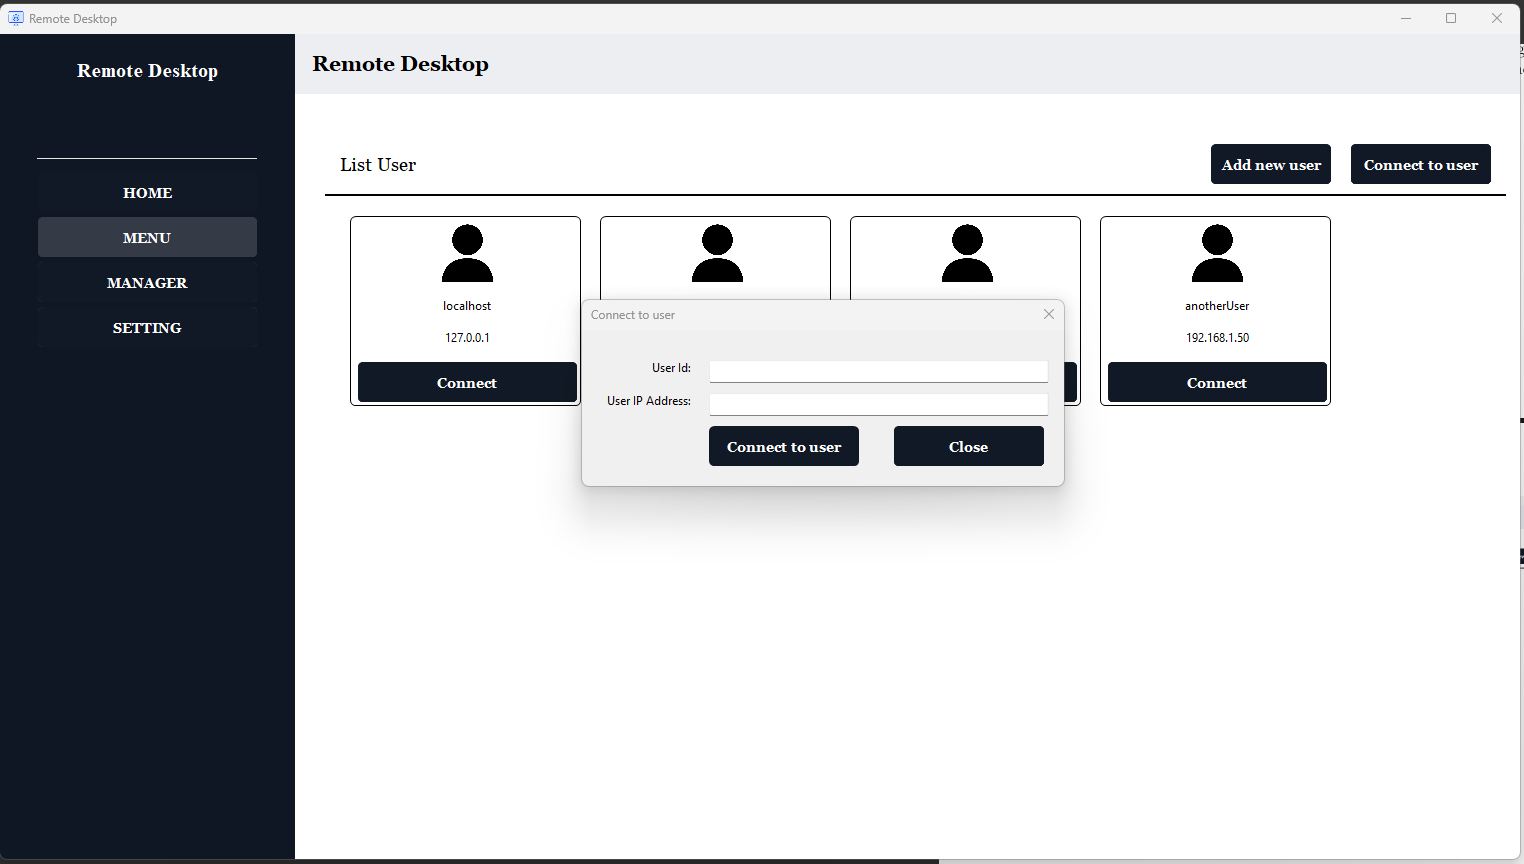
\includegraphics[scale=0.4]{ConnectToUserBox}}
	\caption{Hộp thoại Add new user}
	\label{fig:ConnectToUserBox}
\end{figure}

Nếu ta sử dụng lựa chọn ``Connect'' bên dưới user cần kết nối trong danh sách User, ta chỉ nhấn vào nút ``Connect'' tương ứng.

Lưu ý về địa chỉ IP khi kết nối :
\begin{itemize}
	\item  Kết nối 2 ứng dụng trên 2 máy khác nhau trong cùng mạng: người dùng phía Client cần biết trước IP của máy Server. IP của máy Server có thể lấy ra bằng lệnh \verb|ipconfig| của \textbf{Command Prompt}.
	\item Kết nối 2 ứng dụng trên cùng 1 máy: ngoài cách trên, còn có thể nhập địa chỉ loopback \textbf{127.0.0.1}. Đây là địa chỉ IP đặc biệt được dùng để tham chiếu đến chính máy tính đang sử dụng. Khi gửi dữ liệu đến địa chỉ loopback, dữ liệu sẽ được gửi và xử lý trên cùng một máy tính mà không cần thông qua mạng vật lý.
\end{itemize}

Sau khi nhập địa chỉ IP thích hợp và nhấn kết nối, sẽ có hai cửa sổ hiện ra với tiêu đề tương ứng là ``Client Logger'' và ``Client Window''. Nếu kết nối thất bại, 2 cửa sổ này sẽ không có thông tin gì trên đó, cửa sổ Logger sẽ không ghi thông tin gì và cửa sổ ``Client Window'' sẽ không hiển thị màn hình của máy Server (Hình \ref{fig:ClientWindowFailed}). Khi gặp trường hợp trên, ta tắt cửa sổ ``Client Window'' để đóng kết nối hiện tại và quay lại cửa sổ Menu sử dụng lệnh ``Connect'' để thiết lập kết nối mới.

\begin{figure}[H]
	\centering{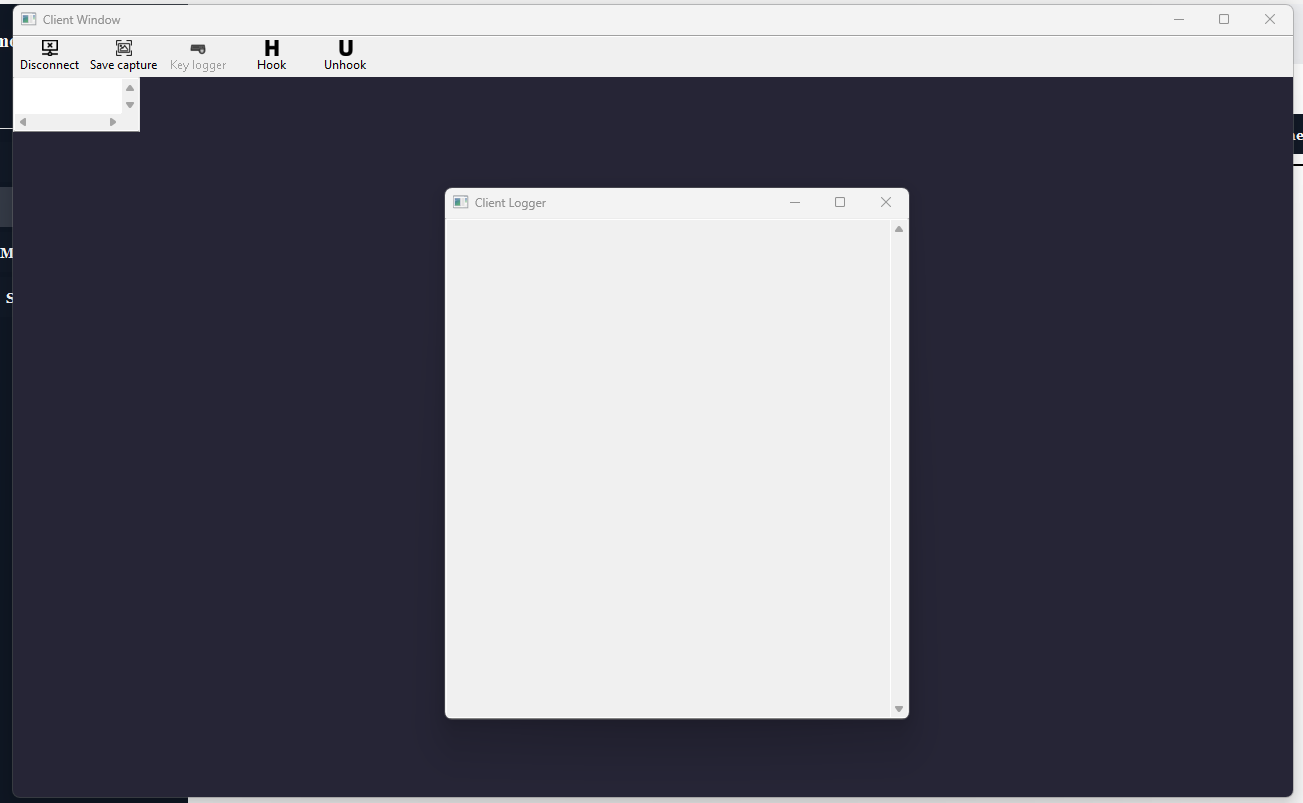
\includegraphics[scale=0.4]{ClientWindowFailed}}
	\caption{Cửa sổ CLient Window khi kết nối không thành công}
	\label{fig:ClientWindowFailed}
\end{figure}

Nếu kết nối thành công, cửa sổ ``Client Window'' sẽ hiển thị màn hình của máy được kết nối, còn cửa sổ ``Client Logger'' sẽ hiển thị thông tin cơ bản của máy Server được kết nối bao gồm địa chỉ IP, địa chỉ MAC và tên cửa sổ của Server. Ở đây thông tin của Server được hiển thị hai lần vì Client thiết lập 2 kết nối đến Server, một cái dùng để nhận hình ảnh và một cái dùng để truyền tín hiệu điều khiển.

Chèn hình ở đây.